\chapter{Implementation der Services am Beispiel \acrshort{lidar}}
Hier gehe ich darauf ein, wie sich das Konzept aus Kapitel \ref{chap:software-design} in Programmcode umsetzen lässt. Dabei versuche ich den Code so einfach wie möglich zu halten, da die Schüler der HFTM parallel erst an Java ausgebildet werden (siehe Anforderungen aus Abschnitt \ref{chap:aufgabenstellung}). Auf Lambda-Ausdrücke wird beispielsweise verzichtet.
\label{chap:beispielimplementation}
\section{Die Library 'GatewayClient'}
Mit der  Java-Library \ctexttt{ch.quantasy.mqtt.gateway} von Reto Koenig \cite{ch.quantasy.mqtt.gateway} lässt sich einfach ein Microservice entwickeln, der sich bereits an das Muster aus Kapitel \ref{sec:isePattern} hält (Event, Intent, Status). Man kann damit keine Messages ins MQTT publizieren die das Muster verletzen.
\begin{figure}[H]
	\centering
	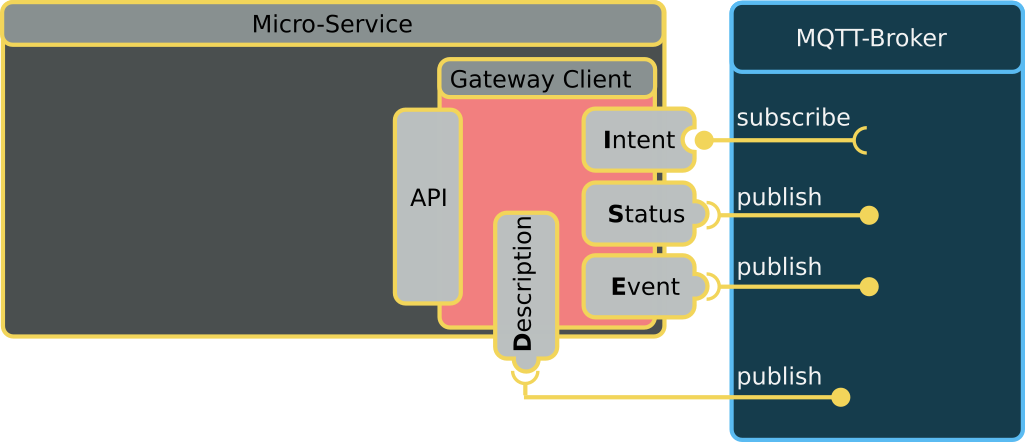
\includegraphics[width=0.6\textwidth]{img/gatewayclient.png}
	\caption{GatewayClient, ch.quantasy.mqtt.gateway\cite{ch.quantasy.mqtt.gateway}}
	\label{fig:gatewayclient}
\end{figure}
In Abbildung \ref{fig:gatewayclient} ist ersichtlich wie die Library die Basis-Topics bzw. \acrshort{api}s in Richtung MQTT-Broker zur Verfügung stellt. Die Idee hinter dem \verb|GatewayClient| ist folgende:
\begin{itemize}
	\item
	Standardisieren der Schnittstelle. Man wird zwar ,,eingeengt'' aber dafür ist die Schnittstelle einheitlich.
	\item
	Serialisierung und übertragen der Java-Objekte auf MQTT in \acrshort{yaml}-Struktur (bei den published Topics)
	\item
	Deserialisierung der YAML-Daten in die ursprünglichen Java-Objekte (bei den subscribed Topics)
	\item
	Bei jedem Verbinden zum MQTT-Broker publiziert der GatewayClient automatisch die ,,\acrshort{api}-Dokumentation''. So ist sofort ersichtlich was für eine Schnittstelle implementiert werden muss um einen weiteren \Gls{servant} an diese Schnittstelle anzuschliessen.
\end{itemize}
\subsection{Service Logik}
An den GatewayClient wird die eigentliche Service Logik angebunden. Im Github-README unterscheidet Reto Koenig\cite{ch.quantasy.mqtt.gateway} dabei wie in Abbildung \ref{fig:microService} ersichtlich zwischen 'Service Logic' und 'Service Source':
\begin{figure}[H]
	\centering
	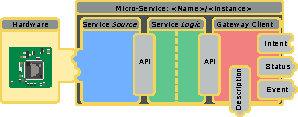
\includegraphics[width=0.6\textwidth]{img/gatewayclient-microservice.pdf}
	\caption{Micro-Service mit GatewayClient \cite{ch.quantasy.mqtt.gateway}}
	\label{fig:microService}
\end{figure}
Was das bedeutet, erklären die nächsten zwei Abschnitte.
\subsubsection{Service Source}
Unter 'Service Source' versteht man die Libraries zu einer bestimmten Hardware. Der Hersteller Tinkerforge\cite{tinkerforge-gmbh} stellt beispielsweise den Java-Code und die Library für die Anbindung ihrer Produkte bereit. Diese Kategorie beinhaltet also die Ansteuerung der Hardware aus Java. Ab diesem Punkt haben wir also Objekte und Klassen, die wir mit der 'Service Logic' ansteuern können.
\subsubsection{Service Logic}
Unter 'Service Logic' versteht man die Logik um beispielsweise einen Sensor, der bereits mittels 'Service Source' von Java aus ansprechbar ist, an den GatewayClient anzubinden.


\section{TiM55x-Service}
Der TiM55x-Service enthält (dh. \verb|import|) zum einen den GatewayClient sowie die Library der HFTM zur Dekodierung und Ansteuerung des \acrshort{lidar}s (also der 'Service Source'). Wir müssen uns folglich also um die 'Service Logic' aus Abbildung \ref{fig:lidarservice} kümmern.
\begin{figure}[H]
	\centering
	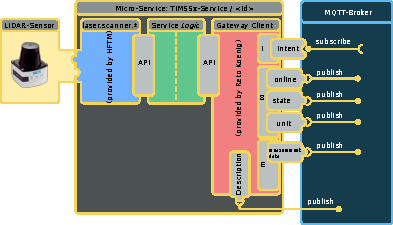
\includegraphics[width=0.6\textwidth]{img/tim55xservice.pdf}
	\caption{TiM55x-Service, Quelle des Diagramm-Templates: \cite{ch.quantasy.mqtt.gateway}}
	\label{fig:lidarservice}
\end{figure}

Der TiM55x-Service ist wie in Abbildung \ref{fig:structure_lidarservice} strukturiert. Die Idee ist, dass der Servant alles aus dem Java-Package 'binding' von unserem Service kennt, solange er auch den GatewayClient verwendet. Darin enthalten ist also die Definition der Schnittstelle und (Objekt-)Strukturen der Daten, die auf dem Event-Bus vorhanden sind.
\begin{figure}[H]
	\centering
	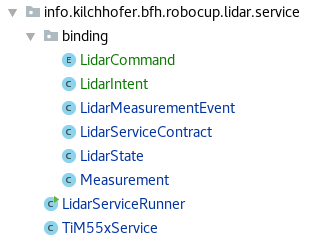
\includegraphics[scale=0.5]{img/tim55x-java-packagestructure.png}
	\caption{TiM55x-Service, Struktur}
	\label{fig:structure_lidarservice}
\end{figure}

Beginnen wir nun mit der Implementation. Der Programmcode in den nachfolgenden Abschnitten ist meist nicht vollständig, damit es übersichtlicher bleibt (mit \ctexttt{// ...} gekennzeichnet). Der vollständige Code dieser Arbeit befindet sich auf Github\cite{github-thesis}. \\
\subsection{Contracts definieren}
Als erstes wird der \Gls{contract} - also die MQTT-Topics und die Struktur der \Gls{payload} - definiert. Dazu wird die abstrakte Basis-Klasse \ctexttt{AyamlServiceContract} wie in Listing \ref{lst:lidarservice-contracts} ersichtlich erweitert.
\begin{lstlisting}[caption={TiM55x-Service - Contracts},label={lst:lidarservice-contracts}]
public class LidarServiceContract extends AyamlServiceContract {
    public final String STATE, MEASUREMENT, STATUS_STATE, EVENT_MEASUREMENT;
    // ...

    public LidarServiceContract(String instanceID) {
        super(ROBOCUP_ROOT_CONTEXT, "Lidar", instanceID);
        STATE = "state";
        MEASUREMENT = "measurement";
        STATUS_STATE = STATUS + "/" + STATE;
        EVENT_MEASUREMENT = EVENT + "/" + MEASUREMENT;
    }

    @Override
    public void setMessageTopics(Map<String, Class<? extends Message>> messageTopicMap) {
        messageTopicMap.put(INTENT, LidarIntent.class);
        messageTopicMap.put(EVENT_MEASUREMENT, LidarMeasurementEvent.class);
        messageTopicMap.put(STATUS_STATE, LidarState.class);
    }
}
\end{lstlisting}
Der TiM55x-Service verwendet also über diesen \Gls{contract} die folgenden \acrshort{mqtt}-\Glspl{topic}:
\begin{itemize}
	\item \texttt{<rootContext>/<baseClass>/U/<instanceID>/I}
	\item \texttt{<rootContext>/<baseClass>/U/<instanceID>/S/state}
	\item \texttt{<rootContext>/<baseClass>/U/<instanceID>/E/measurement}
\end{itemize}
und durch Vererbung:
\begin{itemize}
	\item \texttt{<rootContext>/<baseClass>/U/<instanceID>/S/connection}
\end{itemize}
, wobei über den Aufruf \ctexttt{super(rootContext: "Robocup", baseClass: "Lidar", instanceID)} die variablen Teile der \Glspl{topic} entsprechend gesetzt werden.

\subsubsection{Events: Messdaten}
Schauen wir uns als Beispiel noch das 'measurement'-\Gls{topic} an. Eine Momentaufnahme des \acrshort{lidar}-Sensors, also einer Messung, beinhaltet 270 Messpunkte mit dieser Struktur:
\begin{lstlisting}[caption={TiM55x-Service - Struktur der Messpunkte},label={lst:tim55x-measurement}]
public class Measurement extends AValidator {
    @Range(from = -45, to = 225)
    public int angle;
    
    @Range(from = 0, to = 10000)
    public int distance;
    
    @Range(from = 0, to = 10000)
    public int rssi;

    public Measurement(int angle, int distance, int rssi){
        this.angle = angle;
        this.distance = distance;
        this.rssi = rssi;
    }
    // ...
}
\end{lstlisting}
Über die Annotations geben wir den Variablen die möglichen Werte vor. Damit werden zum einen beim Aufstarten die \Gls{description}-Topics korrekt abgefüllt und zum anderen lassen sich die Empfangenen Werte mit dem \Gls{gatewayclient} validieren (optional). So kann man beispielsweise bestimmen, ob nicht valide Werte weiterverarbeitet werden oder nicht.
Die obigen Messpunkte einer Messung werden in einer Liste als 'LidarMeasurementEvent' übermittelt:
\begin{lstlisting}[caption={TiM55x-Service - Struktur des 'LidarMeasurementEvent'},label={lst:tim55x-measurementEvent}]
public class LidarMeasurementEvent extends AnEvent{
    @ArraySize(min = 1, max = 270)
    private ArrayList<Measurement> measurements;
    
    public LidarMeasurementEvent(ArrayList<Measurement> measurements) {
        this.measurements = measurements;
    }
    // ...
}
\end{lstlisting}

\subsubsection{Intent}
Als Intent bietet der TiM55x-Service an eine Einzel-Messung auszuführen, eine kontinuierliche Messung zu starten und diese zu stoppen. Diese drei Aktionen bietet die Library der HFTM zur Zeit an.
\begin{lstlisting}[caption={TiM55x-Service - Struktur des 'LidarIntent'},label={lst:tim55x-intent}]
import ch.quantasy.mqtt.gateway.client.message.AnIntent;
import ch.quantasy.mqtt.gateway.client.message.annotations.Nullable;

public class LidarIntent extends AnIntent {
    @Nullable
    public LidarCommand command;
    
    //..
}
\end{lstlisting}
LidarCommand ist dabei lediglich ein Enum:
\begin{lstlisting}[caption={TiM55x-Service - Struktur des 'LidarCommand'},label={lst:tim55x-lidarCommand}]
public enum LidarCommand {
    START_CONTINUOUS_MEASUREMENT, STOP_CONTINUOUS_MEASUREMENT, SINGLE_MEASUREMENT
}
\end{lstlisting}

\subsubsection{Status: Laser- / \acrshort{lidar}-State}
Im Status-Topic bietet der TiM55x-Service zusätzlich zum vererbten ConnectionStatus noch den Laser-State an. Das Problem ist hier, dass im Contract die Klasse \ctexttt{IScanOperator.State} verwendet wird, die aus einer Dependency kommt (Service Source). Die Servants im System sollten diese hardwarespezifische Klasse eigentlich nicht kennen und sollten auch nicht abhängig davon sein. So sind sie aber leider davon abhängig und benötigen diese Library über die Paketierung als \ctexttt{jar-with-dependencies}. Dies wird im Kapitel \ref{sec:separatebindings} weiter diskutiert.
\begin{lstlisting}[caption={TiM55x-Service - Struktur des 'LidarState'},label={lst:tim55x-lidarState}]
//..
import laser.scanner.IScanOperator;

public class LidarState extends AStatus{
    public IScanOperator.State state;

    public LidarState(IScanOperator.State state) {
        this.state = state;
    }

    public LidarState() {
    }
}
\end{lstlisting}

\subsubsection{Übersicht über den fertigen Contract}
Der Programmcode von oben führt uns zu dieser Struktur für den TiM55x-ServiceContract (Abbildung \ref{fig:tim55x-binding-overview}). Das Muster (Event, Intent Status) ist hier gleich ersichtlich.
\begin{figure}[H]
	\centering
	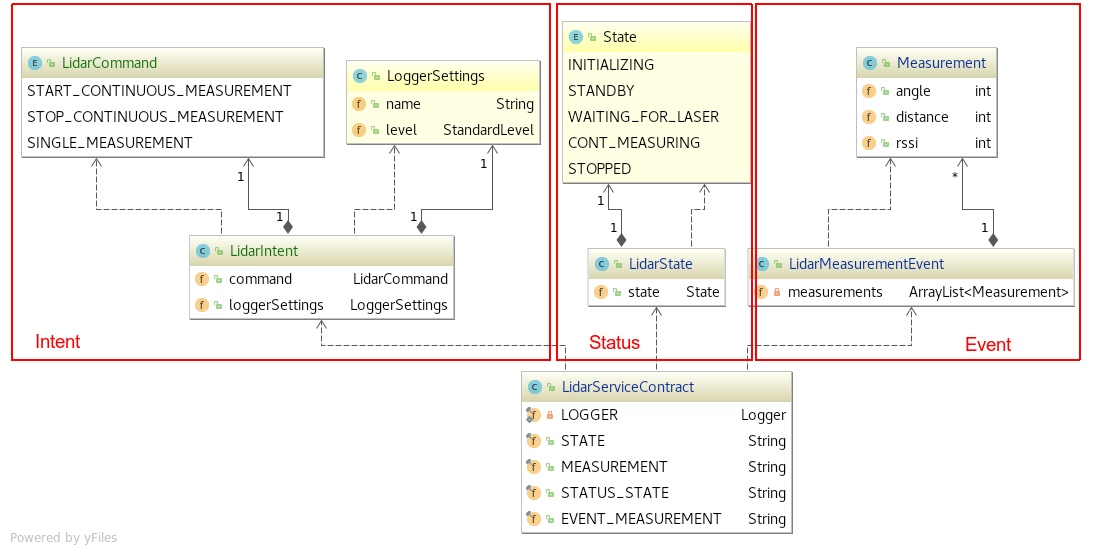
\includegraphics[width=0.7\textwidth]{img/tim55x-binding-overview.png}
	\caption{Übersicht über das Zusammenspiel des Contracts im Package binding}
	\label{fig:tim55x-binding-overview}
\end{figure}

\subsection{Service Logik implementieren}
\label{sec:service-logik-tim55x}
Die nachfolgenden Code-Snippets aus Listing \ref{lst:TiM55x-service} zeigen den Aufbau des TiM55x-Service. Der GatewayClient wird über \ctexttt{<LidarServiceContract>} mit dem \Gls{contract} instantiiert, damit er die Schnittstelle kennt. Bei den Zeilen mit \ctexttt{IScanListener ... }, \ctexttt{IScanOperator ...} sowie \ctexttt{new TiM55x(...)} sieht man die Anbindung an die Sensor-Libary. Andersherum bei \ctexttt{MessageReceiver} und \ctexttt{gatewayClient.subscribe} die Anbindung mit dem GatewayClient an \acrshort{mqtt}. Der Code zeigt also schön, wie die 'Service Logic' beide ,,Welten'' zusammenklebt.

\lstinputlisting[caption={Aufbau TiM55x-Service},language=Java,label={lst:TiM55x-service}]{listings/lidarservice_new.java}

Beim Verarbeiten des Intents wird es spannend. Wir können mit dem GatewayClient ein Set von Messages erhalten - sprich wir können mehrere Intents zum exakt gleichen Zeitpunkt erhalten. Wir nehmen hier einfach den letzten (also den neuesten) im Set. Wie sich ein Service diesbezüglich verhalten soll, muss je nach Situation geklärt werden. Hier wird es sicherlich keinen Sinn machen, den Laser beispielsweise zu aktivieren und gleich wieder zu deaktivieren. Oder wenn zwei Anfragen für eine Einzel-Messung kommen, reicht es auch, die letzte Anfrage auszuführen, es hören ja alle zu und bekommen die Messwerte geliefert.

\subsection{Beispiel-Message am MQTT-Broker}
Der Programmcode aus den Abschnitten oben, wird folgende Nachrichten auf dem MQTT-Broker erzeugen:
\begin{lstlisting}
Robocup/Lidar/U/127.0.0.1@kicm-fedora.localdomain/I ---
- timeStamp: 1528384864556686000
  command: "SINGLE_MEASUREMENT"

Robocup/Lidar/U/127.0.0.1@kicm-fedora.localdomain/E/measurement ---
- timeStamp: 1528384864699874545
  measurements:
- angle: -45
  distance: 278
  rssi: 154
- angle: -44
  distance: 288
  rssi: 157
  .
  . (nicht komplett)
  .
- angle: 224
  distance: 1130
  rssi: 182
\end{lstlisting}

\subsection{Tests mit JUnit}
Der TiM55x-Service verwendet als '\Gls{service-source}' die Library der HFTM. Theoretisch müsste hier also die '\Gls{service-logic}' per Unit-Test getestet werden. Ein einfacher Unittest ist aber ohne die beiden Libraries '\Gls{service-source}' und '\Gls{gatewayclient}' zu mocken fast nicht möglich und auch nicht sehr aussagekräftig. Deshalb werden am Service lediglich Service-Tests mit JUnit durchgeführt. Dies geschieht automatisch in der Maven Lifecycle-Phase \textit{integration-test}.
\subsubsection{Service-Test initialisieren}
Initialisiert wird das Setup wie folgt:
\begin{lstlisting}[caption={Service-Test Setup für den TiM55x-Service},label={lst:integrationstest-tim55x-setup}]
public class TiM55xServiceIntegrationTest {
    // ..
    static int LIDAR_PORT = 2112;
    static String LIDAR_IP = "127.0.0.1";
    static String MQTT_BROKER = "tcp://127.0.0.1:11234";
    //.. 
    @BeforeAll
    public static void setUpBeforeClass() {
        mqttURI = URI.create(MQTT_BROKER);
        //..
        try {
            // Embedded Broker
            // https://github.com/andsel/moquette/blob/master/
            // embedding_moquette/src/main/java/io/moquette/
            // testembedded/EmbeddedLauncher.java
            EmbeddedBrokerLauncher embeddedBrokerLauncher = new EmbeddedBrokerLauncher();

            // Start Hardware Mock
            Runnable r = new Runnable() {
            @Override
                public void run() {
                    try {
                        new HardwareMock(LIDAR_PORT);
                    } catch (InterruptedException e) {
                        LOGGER.error("InterruptedException: ", e);
                    }
                }
            };
            new Thread(r).start();
            Thread.sleep(2000);

            // GatewayClient
            gatewayClient = new GatewayClient<TiM55xServiceTestContract>(mqttURI, mqttClientName, new TiM55xServiceTestContract(instanceName));
            gatewayClient.connect();
            Thread.sleep(1000);
        } catch (Exception e) {
            fail("Exception during Setup");
        } 
    }
    
    // Hier folgen die Test cases
}
\end{lstlisting}
Wir starten also gleich zwei Umsysteme damit - einen Mock-Service (siehe Kapitel \ref{chap:tim-mock}) und einen MQTT-Broker (Moquette MQTT broker \cite{moquette-mqtt-broker}). Damit lässt sich das ganze auch wieder automatisieren. Wir müssen also nicht von Hand erst einen Sensor ans Netzwerk anschliessen, den Broker starten und danach erst den Test ausführen. Der JUnit-Test erledigt alles für uns. So wird sichergestellt, dass bei jedem Release aussagekräftige Tests durchgeführt werden. Bei einer Anpassung am Code, sieht man also sofort, dass etwas nicht mehr stimmt.

\subsubsection{Test-Szenario 'TiM55x-Service starten'}
Kommen wir also zum ersten Test-Szenario: den TiM55x-Service starten.
\begin{lstlisting}[caption={TiM55x Startup-Test}]
@Test
@DisplayName("Start TiM55x Service")
public void bringTiM55xServiceUp() {
    try {
        tiM55xService = new TiM55xService(mqttURI, "SomeTestingWithTiM55x", "SomeTestingWithTiM55x",LIDAR_IP, LIDAR_PORT);
        Thread.sleep(2000);
    } catch (Exception e) {
        fail("Exception during TiM55x Startup");
    }
}
\end{lstlisting}
Startet der Service ohne Exception nehmen wir an, dass er korrekt aufgestartet ist. Denn er wirft sofort Exceptions wenn die Sensor- oder \acrshort{mqtt}-Seite nicht da ist.

\subsubsection{Test-Szenario 'Status-Topic prüfen'}
Jetzt wird es spannender. Wir prüfen nun, wie sich der Status vom TiM55x-Service verhält. Dazu abonnieren wir das entsprechende Topic beim MQTT-Broker und prüfen ob der Status auf  'online' gewechselt hat (\ctexttt{assertEquals(...)}). Falls nicht, schlägt dieser Test fehl.

Das Problem ist, dass die Tests warten müssen, bis wir eine Antwort über den \acrshort{mqtt}-Broker erhalten. Es ist also nicht ein synchroner Aufruf wie beispielsweise bei einer bekannten HTTP-Anfrage (Request, Response), sondern eben asynchron (Publish, Subscribe, siehe \ref{sec:publish-subscribe}). Das heisst für uns, dass die Antwort irgendwann kommen kann und nicht direkt beim Aufruf von \ctexttt{gatewayClient.subscribe(...)}. Deshalb bauen wir einen \ctexttt{CountDownLatch} ein, den wir auf 1 stellen. Beim Empfangen (\texttt{messageReceived}) dekrementieren wir dem Counter. Die Zeile \ctexttt{latch.await(100, TimeUnit.SECONDS)} wartet bis dieser Counter auf 0 steht und blockiert ansonsten maximal für 100 Sekunden, bevor der Test ausgewertet (\texttt{assertEquals}) wird.

\begin{lstlisting}
@Test
@DisplayName("Subscription to Connection Status Topic")
public void subscribeStatus() throws InterruptedException {
    CountDownLatch latch = new CountDownLatch(1);

    MessageReceiver messageReceiver = new MessageReceiver() {
        @Override
        public void messageReceived(String topic, byte[] payload) throws Exception {
            LOGGER.trace("Payload: " + new String(payload));
            resultConnectionStatus = (ConnectionStatus) gatewayClient.toMessageSet(payload, ConnectionStatus.class).last();
            latch.countDown();
        }
    };

    this.gatewayClient.subscribe(tempLidarServiceContract.STATUS_CONNECTION, messageReceiver);
    latch.await(100, TimeUnit.SECONDS);
    assertEquals("online", resultConnectionStatus.value);
}
\end{lstlisting}

\section{ConsoleUI-Service}
\label{sec:ConsoleUI-Service}
Nachdem wir nun im Grundsatz wissen, wie ein Service aufgebaut wird, fallen die Erklärungen in diesem Abschnitt geringer aus.\\ Ein einfacher UI Service soll uns ein Command Line Interface zur Verfügung stellen. Die Struktur sieht analog vom TiM55x-Service aus:
\begin{figure}[H]
	\centering
	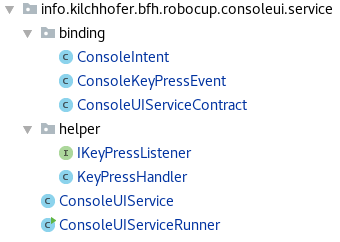
\includegraphics[scale=0.5]{img/consoleui-java-packagestructure.png}
	\caption{ConsoleUI-Service, Struktur}
	\label{fig:structure_consoleuiservice}
\end{figure}
\subsection{Contracts definieren}
\subsubsection{Event}
Der Service wird jeden Tastendruck als einzelnen Event publizieren (Listing \ref{lst:consoleui-KeyPressEvent}).
\begin{lstlisting}[caption={KeyPressEvent für den ConsoleUI-Service},label={lst:consoleui-KeyPressEvent}]
public class ConsoleKeyPressEvent extends AnEvent{
    @StringForm
    @StringSize (min=1, max=1)
    public Character character;

    public ConsoleKeyPressEvent(Character character){
        this.character = character;
    }

    public ConsoleKeyPressEvent() {
    }
}
\end{lstlisting}
\subsubsection{Intent}
Als Intent bietet der Service an, einen String ins Terminal zu schreiben (Listing \ref{lst:consoleui-intent}). Hier ist zusätzlich noch ein weiterer Intent verfügbar: loggerSettings. Damit kann man den Loglevel zur Laufzeit ändern. Er soll lediglich als Beispiel dienen, aber trotzdem eine sinnvolle Funktion anbieten. Über die Annotations wird in diesem \Gls{contract} festgelegt, dass sie nicht vorhanden sein müssen (\texttt{@Nullable}). Wir könnten also auch einen Intent an diesen Service senden, der nur einen Timestamp enthält. Diesen erzwingt der GatewayClient.
\begin{lstlisting}[caption={Intent für den ConsoleUI-Service},label={lst:consoleui-intent}]
public class ConsoleIntent extends AnIntent{
    @Nullable
    public LoggerSettings loggerSettings;

    @Nullable
    @StringForm
    public String consoleMessage;

    public ConsoleIntent(String consoleMessage){
        this.consoleMessage = consoleMessage;
    }

    public ConsoleIntent(){
    }
}
\end{lstlisting}
\subsection{Service Logik implementieren}
Die Logik ist wieder analog wie beim TiM55x-Service: wir haben einen Teil der ankommende Intents verarbeitet und einen keyPressListener, der bei jedem Tastendruck einen Event zum \acrshort{mqtt}-Broker sendet.
\begin{lstlisting}[caption={Service Logik für den ConsoleUI-Service},label={lst:consoleui-service-logic}]
//..
// Intent Handling
this.intentReceiver = new MessageReceiver() {
    @Override
    public void messageReceived(String topic, byte[] payload) throws Exception {
        for(ConsoleIntent intent : gatewayClient.toMessageSet(payload, ConsoleIntent.class)){
            if (intent.consoleMessage != null){
                System.out.println(intent.consoleMessage);
            }

            if (intent.loggerSettings != null){
                intent.loggerSettings.configure();
            }
        }
    }
};
this.gatewayClient.connect();
this.gatewayClient.subscribe(gatewayClient.getContract().INTENT + "/#", this.intentReceiver);

// Event / Console Handling
IKeyPressListener keyPressListener = new IKeyPressListener() {
    @Override
    public void keyPressed(Character character) {
        gatewayClient.readyToPublish(gatewayClient.getContract().EVENT_KEYPRESS, new ConsoleKeyPressEvent(character));
    }
};
keyPressHandler = new KeyPressHandler(keyPressListener);
Thread keyPressHandlerThread = new Thread(keyPressHandler);
keyPressHandlerThread.start();
\end{lstlisting}

\section{TiM55x-zu-ConsoleUI-Servant}
Im Abschnitt \ref{sec:Architektur} wird erläutert, dass Services untereinander keine Abhängigkeit haben. Der Servant aber hat nun Abhängigkeiten zu den bedienenden Services. So müssen wir also diese Abhängigkeiten im POM (\texttt{pom.xml}) spezifizieren, damit wir den Inhalt der entsprechenden Jars auf dem ClassPath zur Verfügung haben und die Bindings benützen können:
\begin{lstlisting}[caption={Dependencies vom TiM55x-zu-UI-Servant},label={lst:servant-dependencies},language={XML}]
<dependency>
  <groupId>info.kilchhofer.bfh</groupId>
  <artifactId>robocup-consoleui-service</artifactId>
  <version>20180607.0</version>
</dependency>
  <dependency>
  <groupId>info.kilchhofer.bfh</groupId>
  <artifactId>robocup-lidar-service</artifactId>
  <version>20180607.0</version>
  <classifier>jar-with-dependencies</classifier>
</dependency>
\end{lstlisting}
\label{sec:servant-dependencies}
Die Übersicht über den Contract vom TiM55x-Service (Abbildung \ref{fig:tim55x-binding-overview}) zeigt, wie die State-Klasse aus der 'Service Source' bis zum Contract / Binding nach vorne durchdrückt. Dies wurde bewusst so beibehalten um dies hier zu diskutieren. Aufgrund dieser Tatsache brauchen wir wie im Listing \ref{lst:servant-dependencies} auf Zeile 10 ersichtlich das Komplette Jar mit allen Dependencies (Fat Jar). Vergleich 20 kB zu 4.2 MB. Das sollten wir also in Zukunft vermeiden und beim Contract nur Objekte definieren, die wir auch im Binding-Package haben.
\begin{lstlisting}[caption={Grössenvergleich Jar zu Fat-Jar vom TiM55x-Service},label={lst:tim55x-service-fat-jar},language={none}]
$ pwd
/home/mkilchhofer/.m2/repository/info/kilchhofer/bfh/robocup-lidar-service/20180612-SNAPSHOT
$ du -h *
4.0K	maven-metadata-local.xml
4.0K	_remote.repositories
20K	robocup-lidar-service-20180612-SNAPSHOT.jar
4.2M	robocup-lidar-service-20180612-SNAPSHOT-jar-with-dependencies.jar
4.0K	robocup-lidar-service-20180612-SNAPSHOT.pom
\end{lstlisting}

\subsection{Contracts definieren überflüssig}
Anders als ein Service muss ein Servant keinen spezifischen \Gls{contract} haben. Deshalb definieren wir einen ,,leeren'' Contract (Listing \ref{lst:emptyContract}). Eigentlich könnten wir den \ctexttt{AyamlServiceContract} direkt verwenden, wenn diese Klasse nicht \ctexttt{abstract} wäre. Natürlich können wir dies auch Anonym im Servant selber umsetzen, aber wir machen es analog den Services, damit ist es Projektweit identisch ist, und wir uns sofort zurecht finden.
\begin{lstlisting}[caption={,,leerer Contract'' für den Servant},label={lst:emptyContract}]
public class ConsoleUIServantContract extends AyamlServiceContract {
    public ConsoleUIServantContract(String instanceID) {
        super(ROBOCUP_ROOT_CONTEXT, "Lidar-ConsoleUI-Servant", instanceID);
    }
    @Override
    public void setMessageTopics(Map<String, Class<? extends Message>> map) {
        // none
    }
}
\end{lstlisting}
Damit kann der Servant lediglich seinen ConnectionStatus publizieren. Natürlich ist es nicht verboten weiteres anzubieten. Wir könnten beispielsweise für eine Monitoring-Software als Status anbieten, ob sich Servant und Service gefunden haben. Oder wie viele Service-Instanzen der Servant bedient. Für uns reicht es aber vorerst aus, mit dem ,,leeren'' und somit generischen Contract zu beginnen.

\subsection{Servant Logik implementieren}
Über den Trick mit \ctexttt{\path{new ConsoleUIServiceContract("+").STATUS_CONNECTION}} (Zeile 18 und 19) lassen wir uns einen String für den Subscribe-Vorgang generieren, der aufgelöst wie folgt aussieht: \\ \ctexttt{Robocup/ConsoleUI/U/+/S/connection}. Das ist also eine Wildcard Subscription. Das heisst, anstelle vom '+'-Zeichen kann alles stehen ausser einem weiteren '/'-Trennzeichen .
Durch diese Subscription bekommen wir die ConnectionStatus-Infos aus allen Instanzen vom Console-UI-Service. Bei drei Instanzen bekämen wir also die Infos aus beispielsweise folgenden Topics:
\begin{itemize}
	\item \texttt{Robocup/ConsoleUI/U/1234@kicm-fedora.localdomain/S/connection}
	\item \texttt{Robocup/ConsoleUI/U/5678@kicm-fedora.localdomain/S/connection}
	\item \texttt{Robocup/ConsoleUI/U/9876@kicm-fedora.localdomain/S/connection}
\end{itemize}

Die Implementierung des eigentlichen Services ist wieder sehr simpel:
\lstinputlisting[caption={Aufbau TiM55x-UI-Servant},language=Java,label={lst:TiM55x-UI-Servant}]{listings/servant.java}

Der Servant hat nun einige \ctexttt{MessageReceiver} mehr als die Services. Grundsätzlich so viele, wie alle Events von den zu bedienenden Services zusammen addiert. Wir wollen ja die publizierten Events und Stati im Servant abonnieren und dem anderen Service im korrekten Format als Intent publizieren.
Schauen wir uns doch mal die einfachen Receiver an:
\subsubsection{Receiver für den Connection-Status einer ConsoleUI-Instanz}
Sobald wir auf dem Topic \ctexttt{Robocup/ConsoleUI/U/+/S/connection} Nachrichten mit \ctexttt{\path{value: "online"}} in der \Gls{payload} erhalten nehmen wir diese Unit bzw. Instanz in eine Liste auf und machen eine spezifische Subscription auf den \texttt{\path{EVENT_KEYPRESS}} dieser Instanz. Wir wollen alle UIs die zuschauen möchten mit den Daten des \acrshort{lidar}s versorgen. An dieser Subscription hängen wir als Callback den \ctexttt{keyPressReceiver} an.
\begin{lstlisting}[language=Java,caption={MessageReceiver für den Connection-Status einer ConsoleUI-Instanz im Servant},label={lst:servant-uiConnectionStatusReceiver}]
this.uiConnectionStatusReceiver = new MessageReceiver() {
    @Override
    public void messageReceived(String topic, byte[] payload) throws Exception {
        LOGGER.trace("uiConnectionStatusReceiver Payload: " + new String(payload));
        ConnectionStatus connectionStatus = gatewayClient.toMessageSet(payload, ConnectionStatus.class).last();
        ConsoleUIServiceContract uiInstanceContract = new ConsoleUIServiceContract(topic, true);

        LOGGER.info("Instance '{}' is now {}", uiInstanceContract.INSTANCE, connectionStatus.value);

        if (connectionStatus.value.equals("online")) {
            gatewayClient.readyToPublish(uiInstanceContract.INTENT, new ConsoleIntent("This is a message from the Servant, we now have a connection together.") );

            uiInstances.add(uiInstanceContract);
            gatewayClient.subscribe(uiInstanceContract.EVENT_KEYPRESS, keyPressReceiver);
        } else {
            uiInstances.remove(uiInstanceContract);
            gatewayClient.unsubscribe(uiInstanceContract.EVENT_KEYPRESS);
        }
    }
};
\end{lstlisting}

In diesem \ctexttt{keyPressReceiver} sehen wir jetzt schön wie der Servants die Eigenheiten der Services ausgleicht. Oben im Abschnitt \ref{sec:ConsoleUI-Service} haben wir ja gelernt, dass der Console-UI-Service lediglich alle Tastendrücke als Event publiziert. Der Servant macht jetzt damit ein Mapping zum TiM55x-Service:
\begin{itemize}
	\item Taste \keystroke{S}: Single (Einzelmessung)
	\item Taste \keystroke{E}: Enable (Start kontinuierliche Messung)
	\item Taste \keystroke{D}: Disable (Stop kontinuierliche Messung)
\end{itemize}
\begin{lstlisting}[language=Java,caption={MessageReceiver für die keyPress-Evemts einer ConsoleUI-Instanz im Servant},label={lst:servant-uiConnectionStatusReceiver}]
this.keyPressReceiver = new MessageReceiver() {
    @Override
    public void messageReceived(String topic, byte[] payload) throws Exception {
        Set<ConsoleKeyPressEvent> consoleKeyPressEvents = gatewayClient.toMessageSet(payload, ConsoleKeyPressEvent.class);
        for (ConsoleKeyPressEvent consoleKeyPressEvent : consoleKeyPressEvents) {
            LOGGER.trace("Event Payload: " + consoleKeyPressEvent.character);
            LidarIntent lidarIntent = new LidarIntent();

            Character receivedChar = toLowerCase(consoleKeyPressEvent.character);
            // Mapping KeyPress (UI) <--> Lidar features
            switch (receivedChar) {
                case 's':
                    lidarIntent.command = LidarCommand.SINGLE_MEASUREMENT;
                    break;
                case 'e':
                    lidarIntent.command = LidarCommand.START_CONTINUOUS_MEASUREMENT;
                    break;
                case 'd':
                    lidarIntent.command = LidarCommand.STOP_CONTINUOUS_MEASUREMENT;
                    break;
                default:
                    LOGGER.warn("Received unknown command '{}'", receivedChar);

            }
            if (lidarIntent.command != null) {
                gatewayClient.readyToPublish(lidarServiceContract.INTENT, lidarIntent);
            }
        }
    }
};
\end{lstlisting}
TODO

\section{TiM55x Mock}
\label{chap:tim-mock}
Um reproduzierbare Messresultate für die automatisierten Tests zu erhalten wurde der TiM55x Sensor gemockt. Dazu wurden einerseits die Dokumente von SICK und der Programmcode der \acrshort{hftm} studiert. Die Kommunikation über das Netzwerk von Sensor zur Applikation gleicht einem einfachen Seriell-Protokoll (RS-232).

\subsection{Telegramme des Sensors verstehen}
Das Dokument ,,Telegram Listing'' \cite{tim55x-telegram-listing} vom Hersteller SICK gibt Aufschluss über den grundsätzlichen Aufbau des Telegramme.
\begin{figure}[H]
	\centering
	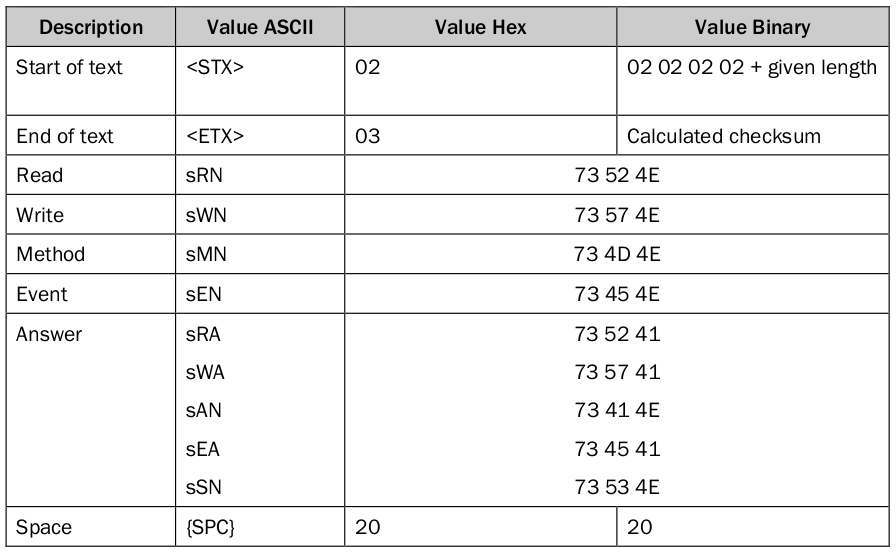
\includegraphics[width=0.5\textwidth]{img/tim55x-telegram-commands.png}
	\caption{Telegram analysieren mit Wireshark}
	\label{fig:tim55x-telegram-commands}
\end{figure}

Um die Kommunikation zwischen Sensor und Applikation zu analysieren wurde mit Wireshark der Netzwerkverkehr aufgezeichnet (Abbildung \ref{fig:tim55x-telegram-wireshark}). Die Anfrage stammt vom SICK eigenen Diagnose-Tool ,,SOPAS Engineering Tool'' und schaltet den Sensor online.
\begin{figure}[H]
	\centering
	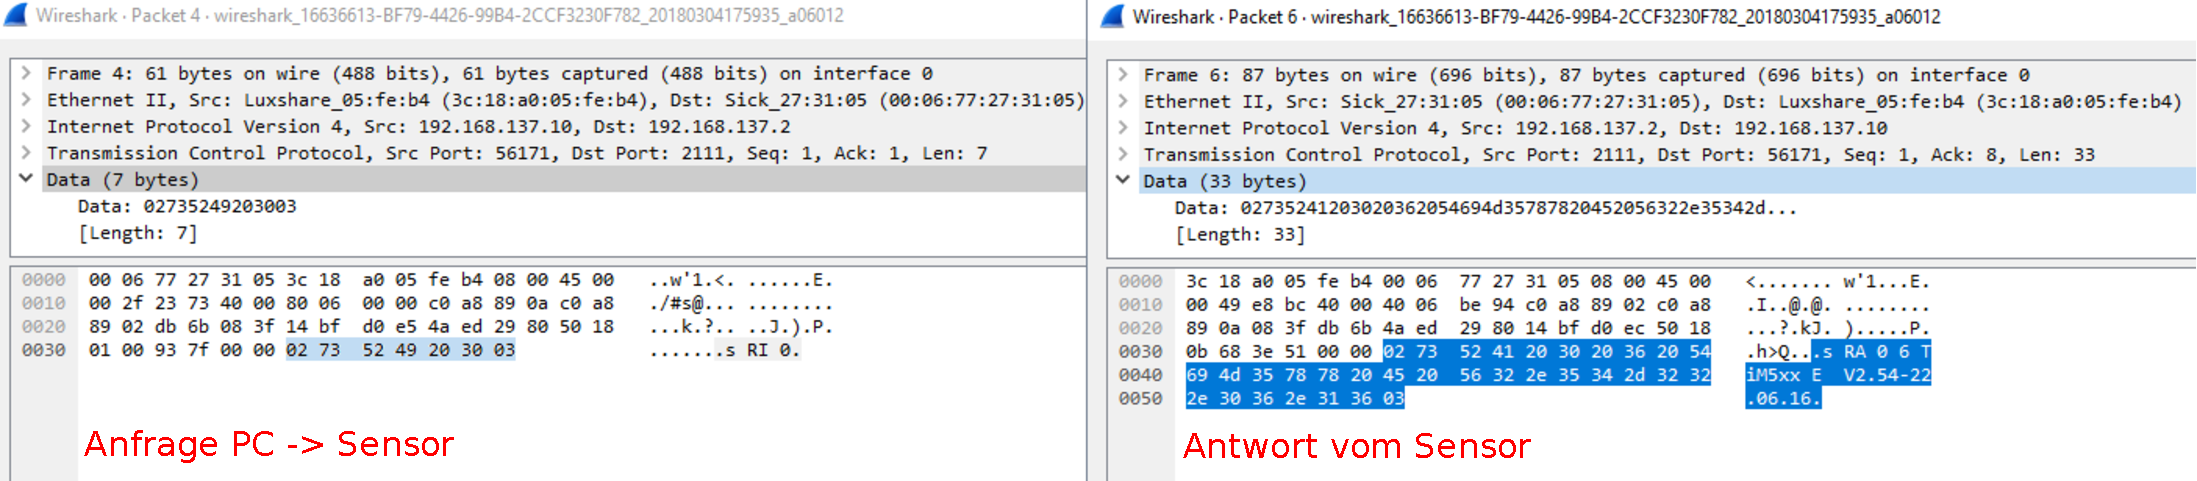
\includegraphics[width=1.0\textwidth]{img/tim55x-telegram-wireshark.pdf}
	\caption{Telegram analysieren mit Wireshark}
	\label{fig:tim55x-telegram-wireshark}
\end{figure}

Die Analyse wurde für alle Aktionen gemacht, welche die von der HFTM zur Verfügung gestellte Library anbietet. Hier eine Zusammenfassung:

\subsubsection{Einzelmessung durchführen (Run single)}
\begin{table}[H]
	\centering
	\begin{tabular}{lp{13cm}} \toprule
		\textbf{Richtung} 	& \textbf{Telegramm-Inhalt}							\\ \midrule
		App -> Sensor		& <STX>sRN LMDscandata<ETX> 							\\ \midrule
		Sensor -> App		& <STX>sRA LMDscandata 1 1 107375C 0 0 2AD8 ... B not defined 0 0 0<ETX>	\\ \bottomrule
	\end{tabular}
	\caption{Kommunikation 'Sensor <--> App' bei Einzelmessung}
	\label{tab:commSingle}
\end{table}

\subsubsection{fortlaufende Messung starten (start)}
\begin{table}[H]
	\centering
	\begin{tabular}{lp{13cm}} \toprule
		\textbf{Richtung} 	& \textbf{Telegramm-Inhalt}							\\ \midrule
		App -> Sensor		& <STX>sEN LMDscandata 1<ETX> 							\\ \midrule
		Sensor -> App		& <STX>sEA LMDscandata 1<ETX>							\\ \midrule
		Sensor -> App (15/s)	& <STX>sSN LMDscandata 1 1 107375C 0 0 E784 ... B not defined 0 0 0<ETX>	\\ \bottomrule
	\end{tabular}
	\caption{Kommunikation 'Sensor <--> App' bei fortlaufender Messung}
	\label{tab:fortlaufendeMessungStart}
\end{table}

\subsubsection{fortlaufende Messung beenden (stop)}
\begin{table}[H]
	\centering
	\begin{tabular}{lp{13cm}} \toprule
		\textbf{Richtung} 	& \textbf{Telegramm-Inhalt}							\\ \midrule
		App -> Sensor		& <STX>sEN LMDscandata 0<ETX> 							\\ \midrule
		Sensor -> App		& <STX>sEA LMDscandata 0<ETX>							\\ \bottomrule
	\end{tabular}
	\caption{Kommunikation 'Sensor <--> App' bei fortlaufender Messung beenden}
	\label{tab:fortlaufendeMessungStop}
\end{table}

\subsection{Implementieren des Mock Services}
Aus diesen Informationen können wir einen simplen Mock-Service implementieren, der lediglich auf diese \underline{drei} Anfragetypen (\ctexttt{sRN LMDscandata}, \ctexttt{sEN LMDscandata 1} und \ctexttt{sEN LMDscandata 0}) von der Applikation hört und jedes mal die gleiche Antwort auf der Anfrage basierend zurück gibt.

\begin{lstlisting}
public class HardwareMock {

    private static ServerSocket serverSocket;
    private static Socket connectionSocket = null;
    private static BufferedReader bufferedReader;
    private static DataOutputStream outputStream;
    private String receivedString = "";

    private final static byte DATA_START = 2;
    private final static byte DATA_END = 3;

    private String singleMeasurementAnswer = "sRA LMDscandata 1 1 107375C 0 0 ...";// nicht komplett
    private String continuousMeasurementAnswer1 = "sEA LMDscandata 1";
    private String continuousMeasurementAnswer2 = "sSN LMDscandata 1 1 107375 ...";// nicht komplett
    private String continuousMeasurementAnswerStop = "sEA LMDscandata 0";

    public HardwareMock (int port, InetAddress bindAddress) throws InterruptedException {
        while (true) {
            try {
                if (serverSocket == null) {
                    LOGGER.info("Opening server socket on '{}:{}'", bindAddress.getHostAddress(), port);
                    serverSocket = new ServerSocket(port, 0, bindAddress);
                }
                if (connectionSocket == null) {
                    LOGGER.info("Start listening for a new connection...");
                    connectionSocket = serverSocket.accept();
                }
                if (bufferedReader == null) {
                    LOGGER.info("Client connected, going on.");
                    bufferedReader = new BufferedReader(new InputStreamReader(connectionSocket.getInputStream()));
                    outputStream = new DataOutputStream(connectionSocket.getOutputStream());
                }
                byte temp = 0;
                while ((temp = (byte) bufferedReader.read()) != -1) {
                    receivedByte(temp);
                    LOGGER.trace("receivedByte ended");
                }
                LOGGER.info("Client disconnected");
                resetSocket();
            } catch (IOException e){
                // ..
            }
        }
    }
}
\end{lstlisting}
Die eigentliche Logik passiert in den Methoden \ctexttt{receivedByte} und \ctexttt{analyseAndPerformAction}. Wir lesen also einfach die Daten auf dem \texttt{InputStream} über den \texttt{BufferedReader} ein und parsen die Bytes sobald wir ein \ctexttt{<ETX>} (end of text) erhalten haben. Danach senden wir sofort beim Erkennen einer bekannten Anfrage (die drei \texttt{if}-Abfragen) die entsprechende Antwort über den \texttt{DataOutputStream} zurück an die Applikation, also dem TiM55x-Service.
\begin{lstlisting}
    public void receivedByte(byte value) {
        LOGGER.trace("receivedByte '{}'", (char)value);
        switch (value){
            case 2:
                this.receivedString = "<STX>";
                LOGGER.info("STX received, clearing String.");
                break;
            case 3:
                this.receivedString = this.receivedString + "<ETX>";
                LOGGER.info("ETX received. String is now: {}", this.receivedString);
                analyseAndPerformAction(this.receivedString);
                break;
            default:
                this.receivedString = this.receivedString + (char)value;
        }
    }

    private void analyseAndPerformAction(String stringToAnalyse){
        if (stringToAnalyse.contains("sRN LMDscandata")) {
            LOGGER.info("Single Scan requested");
            try {
                outputStream.write(DATA_START);
                outputStream.write(singleMeasurementAnswer.getBytes());
                outputStream.write(DATA_END);
                outputStream.flush();
            } catch (IOException e) {
                LOGGER.error("Single Scan error occurred", e);
                return;
            }
         }

         if (stringToAnalyse.contains("sEN LMDscandata 1")) {
             // ..
         }

         if (stringToAnalyse.contains("sEN LMDscandata 0")) {
             // ..
         }

    }
\end{lstlisting}